\chapter{Classificazione dei Design Pattern per Smart-Contract}
I design pattern adottati nello sviluppo di smart-contract possono essere classificati in diversi tipi, alcuni descritti in \cite{9089272} e \cite{9050163}, ognuno dei quali caratterizza un aspetto specifico della lifecycle del contratto:

\begin{itemize}
	\item \textit{Authorization}: relativi alla gestione dell'accesso alle funzionalità del contratto;
	\item \textit{Behavioral}: relativi a meccanismi di supporto per il corretto svolgimento delle funzionalità del contratto;
	\item \textit{Gas Economic}: relativi a meccanismi per ridurre il consumo di \textit{gas} durante l'esecuzione delle funzionalità del contratto;
	\item \textit{Lifecycle}: relativi alla a meccanismi per la creazione e la distruzione del contratto;
	\item \textit{Maintenance}: relativi a meccanismi di supporto per la manutenzione del contratto;
	\item \textit{Security}: relativi a meccanismi per la mitigazione di vulnerabilità di sicurezza note;
\end{itemize}
\textit{Essendo Solidity un linguaggio di programmazione tutt'ora in sviluppo, quindi soggetto a cambiamenti, e le pubblicazioni, scientifiche e di programmatori, alquanto datate, tutti i design pattern individuati sono stati aggiornati dal punto di vista sintattico per essere compatibili con la versione 0.8.0.0 o superiore di Solidity}. 
\newpage
{\section{Authorization Design Pattern}
La blockchain Ethereum non implementa meccanismi di autenticazione o di permessi per consentire l'accesso a specifiche funzionalità di un contratto solo nel caso in cui vengano soddisfatte determinate condizioni. Per la natura della blockchain, ogni funzione definita con visibilità pubblica può essere invocata da qualsiasi utente.\par
Gli \textit{Authorization Design Pattern} propongono meccanismi atti a limitare l'esecuzione delle funzionalità di un contratto.\par
Si individuano i seguenti design pattern: \textit{Access Restriction} e \textit{Ownership}.
{\subsection{Access Restriction Pattern}
	L'\textit{Access Restriction} pattern propone un meccanismo per introdurre dei controlli di prerequisiti nella logica del contratto.\par
	Il meccanismo proposto si basa sul concetto di \textit{function modifiers} presente in Solidity, che permette di definire dei controlli che possono essere eseguiti prima o dopo l'esecuzione del corpo della funzione a cui viene applicato il \textit{modifier}.
	\begin{table}[H]
		\centering
		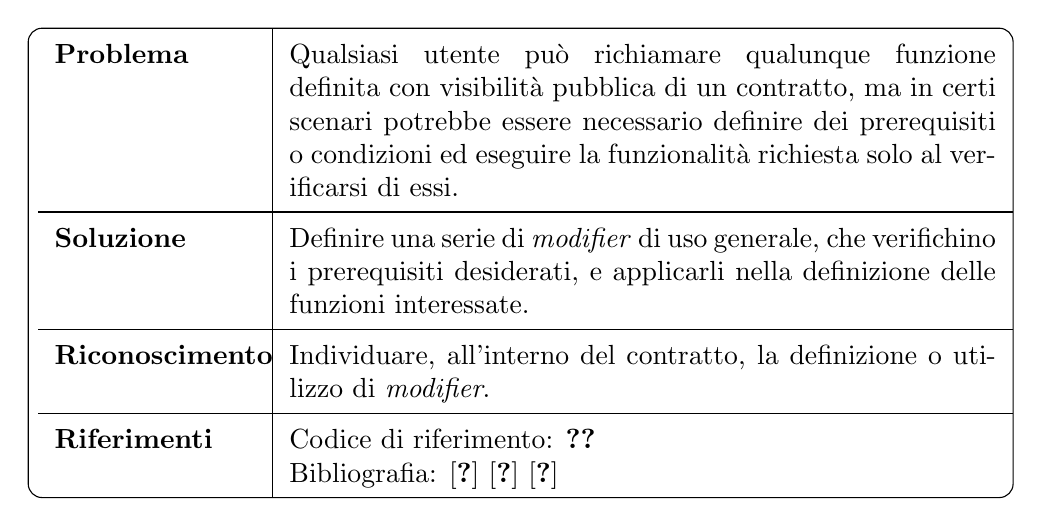
\begin{tikzpicture}
			\node (table) [inner sep=0pt] {
				\def\arraystretch{1.5}
				\begin{tabular}{p{0.21\linewidth} | p{0.74\linewidth}}
					\textbf{Problema} & {Qualsiasi utente può richiamare qualunque funzione definita con visibilità pubblica di un contratto, ma in certi scenari potrebbe essere necessario definire dei prerequisiti o condizioni ed eseguire la funzionalità richiesta solo al verificarsi di essi.} \\ \hline
					\textbf{Soluzione} & {Definire una serie di \textit{modifier} di uso generale, che verifichino i prerequisiti desiderati, e applicarli nella definizione delle funzioni interessate.} \\ \hline
					\textbf{Riconoscimento} & {Individuare,  all'interno del contratto, la definizione o utilizzo di \textit{modifier}.} \\ \hline
					\textbf{Riferimenti} & {Codice di riferimento: \ref{appendix:access_restriction} \newline Bibliografia: \cite{maxwoe} \cite{cjgdev} \cite{fravoll}} \\
				\end{tabular}
			};
			\draw [rounded corners=.5em] (table.north west) rectangle (table.south east);
		\end{tikzpicture}
		\caption{Specifiche dell'Access Restriction Pattern}
	\end{table}
}
\newpage
{\subsection{Ownership Pattern}
L'\textit{Ownership} pattern propone un meccanismo per riservare al proprietario di uno smart-contract l'esecuzione di funzionalità critiche, a cui l'utente finale non deve avere accesso.\par
Opzionalmente, possono essere implementati anche meccanismi di supporto per l'operazione di trasferimento del titolo di proprietario.\par
Questo design pattern può essere considerato come un caso specifico di Access Restriction.
\begin{table}[H]
	\centering
	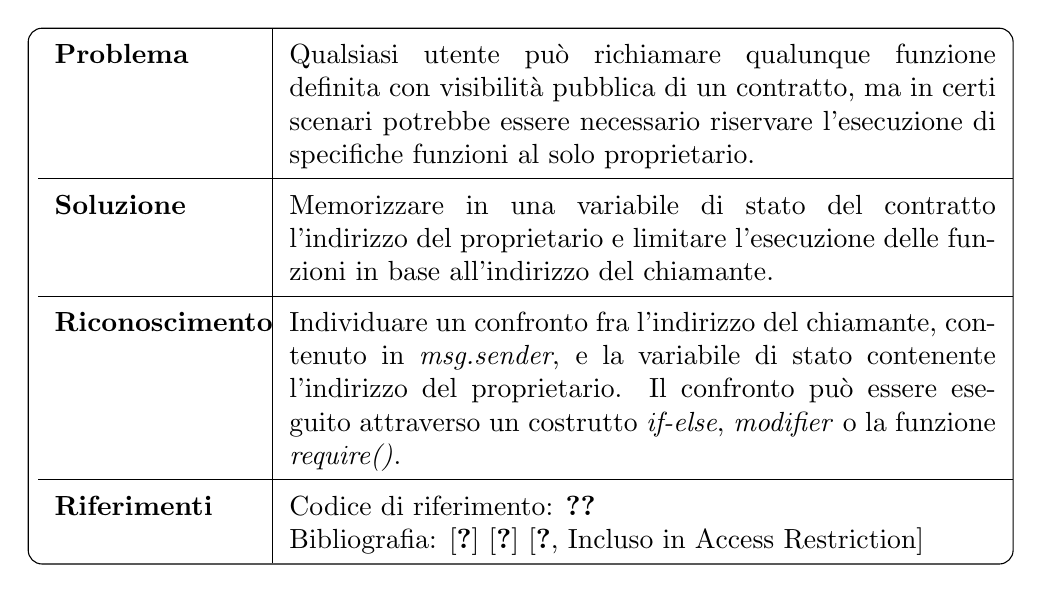
\begin{tikzpicture}
		\node (table) [inner sep=0pt] {
			\def\arraystretch{1.5}
			\begin{tabular}{p{0.21\linewidth} | p{0.74\linewidth}}
				\textbf{Problema} & {Qualsiasi utente può richiamare qualunque funzione definita con visibilità pubblica di un contratto, ma in certi scenari potrebbe essere necessario riservare l'esecuzione di specifiche funzioni al solo proprietario.} \\ \hline
				\textbf{Soluzione} & {Memorizzare in una variabile di stato del contratto l'indirizzo del proprietario e limitare l'esecuzione delle funzioni in base all'indirizzo del chiamante.} \\ \hline
				\textbf{Riconoscimento} & {Individuare un confronto fra l'indirizzo del chiamante, contenuto in \textit{msg.sender}, e la variabile di stato contenente l'indirizzo del proprietario. Il confronto può essere eseguito attraverso un costrutto \textit{if-else}, \textit{modifier} o la funzione \textit\mbox{\textit{require()}}.} \\ \hline
				\textbf{Riferimenti} & {Codice di riferimento: \ref{appendix:ownership} \newline Bibliografia: \cite{maxwoe} \cite{cjgdev} \cite[Incluso in Access Restriction]{fravoll}} \\
			\end{tabular}
		};
		\draw [rounded corners=.5em] (table.north west) rectangle (table.south east);
	\end{tikzpicture}
	\caption{Specifiche dell'Ownership Pattern}
\end{table}
}
}
\newpage
{\section{Behavioral Design Pattern}
I \textit{Behavioral design pattern} propongono funzionalità e meccanismi di supporto per facilitare lo svolgimento delle operazioni del contratto.\par
Si individuano i seguenti design pattern: \textit{Commit \& Reveal}, \textit{Guard Check}, \textit{Oracle}, \textit{Pull Payment (Pull over Push)}, \textit{Randomness} e \textit{State Machine Pattern}.
{\subsection{Commit and Reveal Pattern}
	Il \textit{Commit and Reveal} pattern propone un meccanismo per consentire agli utenti di uno smart-contract di attenersi a un valore tenendolo nascosto agli altri con la possibilità di rivelarlo in seguito.
	\begin{table}[H]
		\centering
		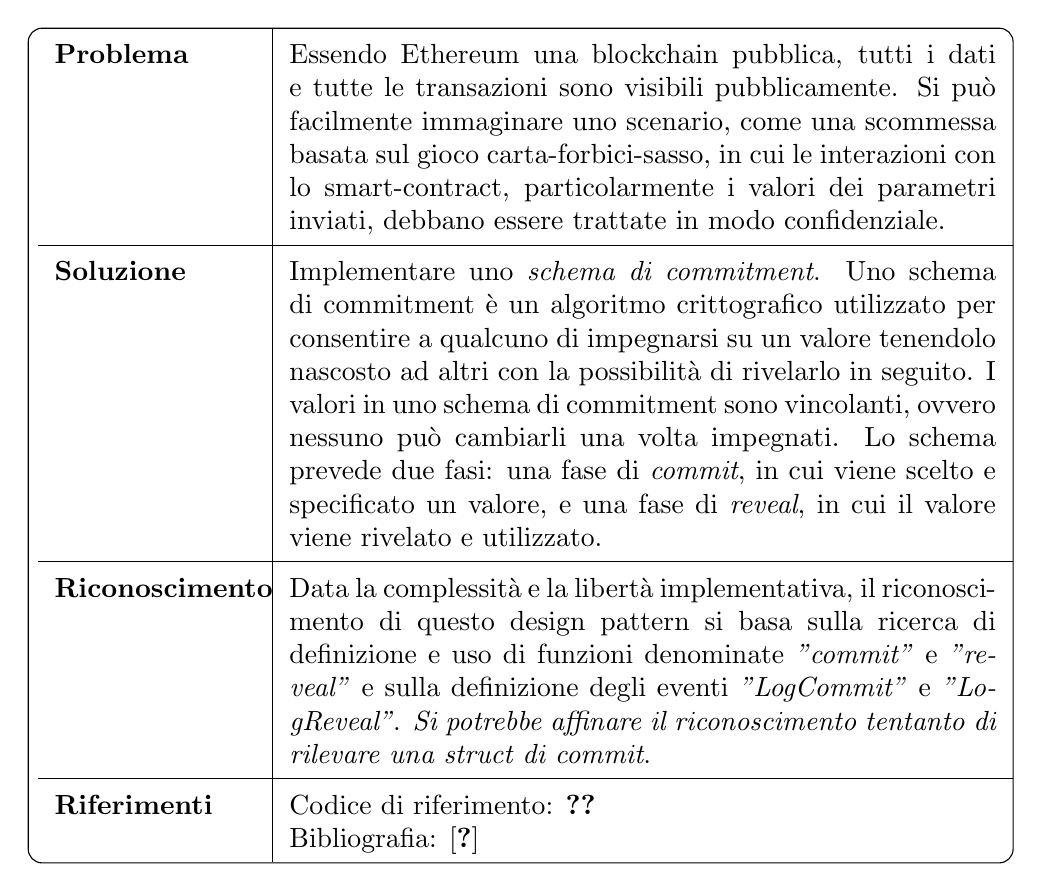
\begin{tikzpicture}
			\node (table) [inner sep=0pt] {
				\def\arraystretch{1.5}
				\begin{tabular}{p{0.21\linewidth} | p{0.74\linewidth}}
					\textbf{Problema} & {Essendo Ethereum una blockchain pubblica, tutti i dati e tutte le transazioni sono visibili pubblicamente. Si può facilmente immaginare uno scenario, come una scommessa basata sul gioco carta-forbici-sasso, in cui le interazioni con lo smart-contract, particolarmente i valori dei parametri inviati, debbano essere trattate in modo confidenziale.} \\ \hline
					\textbf{Soluzione} & {Implementare uno \textit{schema di commitment}. Uno schema di commitment è un algoritmo crittografico utilizzato per consentire a qualcuno di impegnarsi su un valore tenendolo nascosto ad altri con la possibilità di rivelarlo in seguito. I valori in uno schema di commitment sono vincolanti, ovvero nessuno può cambiarli una volta impegnati. Lo schema prevede due fasi: una fase di \textit{commit}, in cui viene scelto e specificato un valore, e una fase di \textit{reveal}, in cui il valore viene rivelato e utilizzato.} \\ \hline
					\textbf{Riconoscimento} & {Data la complessità e la libertà implementativa, il riconoscimento di questo design pattern si basa sulla ricerca di definizione e uso di funzioni denominate \textit{"commit"} e \textit{"reveal"} e sulla definizione degli eventi \textit{"LogCommit"} e \textit{"LogReveal"}. \textit{Si potrebbe affinare il riconoscimento tentanto di rilevare una struct di commit}.} \\ \hline
					\textbf{Riferimenti} & {Codice di riferimento: \ref{appendix:commit_and_reveal} \newline Bibliografia: \cite{maxwoe}} \\
				\end{tabular}
			};
			\draw [rounded corners=.5em] (table.north west) rectangle (table.south east);
		\end{tikzpicture}
		\caption{Specifiche del Commit and Reveal Pattern}
	\end{table}
}
\newpage
{\subsection{Guard Check}
	Nella blockchain Ethereum non vi sono regolatori o mediatori, ma vi è necessità di controlli per assicurare che lo smart-contract funzioni come previsto.\par
	Il \textit{Guard Check} pattern propone un meccanismo per assicurarsi che il comportamento del contratto sia quello previsto, che i parametri di input siano validi e che in caso di errore lo stato interno del contratto venga ripristinato al momento precedente l'esecuzione della funzione.
	\begin{table}[H]
		\centering
		\begin{tikzpicture}
			\node (table) [inner sep=0pt] {
				\def\arraystretch{1.5}
				\begin{tabular}{p{0.21\linewidth} | p{0.74\linewidth}}
					\textbf{Problema} & {Uno smart-contract dovrebbe verificare tutti i prerequisiti della funzionalità richiesta e procedere solo se tutto è come previsto. In caso di errori, il contratto dovrebbe ripristinare tutte le modifiche apportate al suo stato.} \\ \hline
					\textbf{Soluzione} & {Per ottenere questi comportamenti, Solidity sfrutta il modo in cui l'EVM gestisce gli errori: per mantenere l'atomicità, tutte le modifiche effettuate vengono annullate e l'intera transazione viene invalidata. Per innescare gli errori, e quindi ripristinare lo stato interno del contratto, Solidity utilizza una serie di eccezioni, ognuna avente un utilizzo specifico:
					\begin{itemize}[leftmargin=5mm, itemsep=0pt]
						\item \textit{assert(condition)}: usato solo per verificare la presenza di errori interni e per controllare gli invarianti (asserzioni sempre vere). Una caratteristica importante è che rimborsa tutto il gas che non è stato consumato fino al momento in cui viene lanciata l'eccezione;
						\item \textit{require(condition)}: usato solo per garantire condizioni valide, come gli input o le variabili di stato del contratto, o per convalidare i valori di ritorno da chiamate a contratti esterni. Una caratteristica importante è che consuma tutto il gas incluso nella transazione;
						\item \textit{revert()}: usato per ripristinare le modifiche apportate allo stato, viene automaticamente lanciato in caso di fallimento da \textit\mbox{require()} o \textit{assert()} ma potrebbe essere utilizzato all'interno di un controllo fatto da un costrutto \textit{if};
					\end{itemize} \vspace{-6mm}}\\ \hline
					\textbf{Riconoscimento} & {Individuare l'utilizzo di una delle eccezioni: \textit{assert(condition)}, \textit\mbox{require(condition)} o \textit{revert()}.} \\ \hline
					\textbf{Riferimenti} & {Codice di riferimento: \ref{appendix:guardcheck} \newline Bibliografia: \cite{fravoll}} \\
				\end{tabular}
			};
			\draw [rounded corners=.5em] (table.north west) rectangle (table.south east);
		\end{tikzpicture}
		\caption{Specifiche del Guard Check Pattern}
	\end{table}
}
{\subsection{Oracle Pattern}
	Gli smart-contract Ethereum non possono ottenere informazioni dal mondo esterno poiché non possono contattarlo, al contrario si affidano al mondo esterno che immette tali informazioni nella blockchain.\par L'\textit{Oracle} pattern propone un meccanismo per permettere a un contratto di ottenere informazioni presenti al di fuori dalla blockchain, spesso necessarie per il corretto funzionamento del contratto.
	\begin{table}[H]
		\centering
		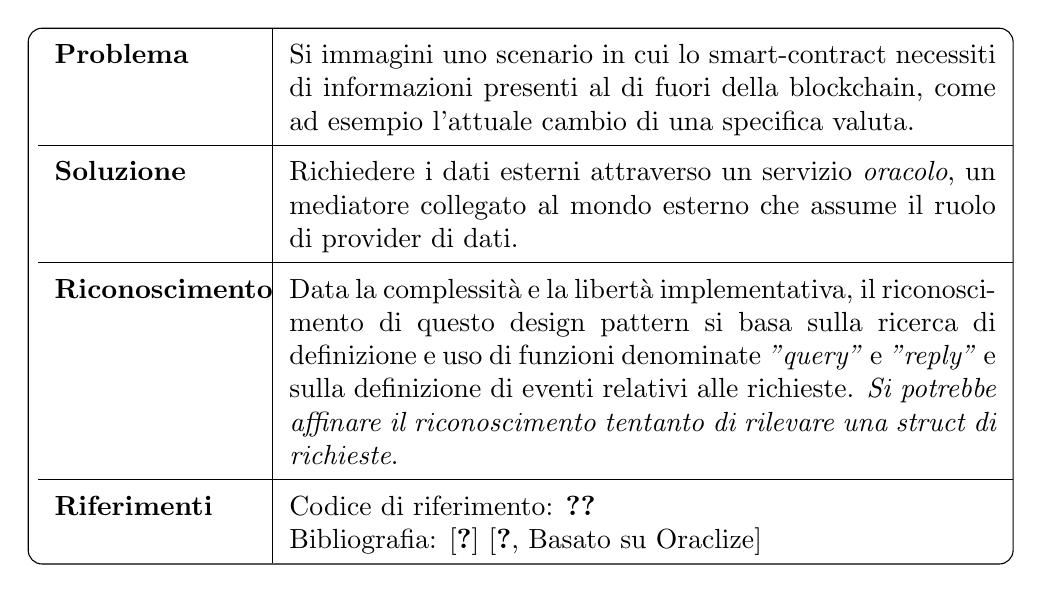
\begin{tikzpicture}
			\node (table) [inner sep=0pt] {
				\def\arraystretch{1.5}
				\begin{tabular}{p{0.21\linewidth} | p{0.74\linewidth}}
					\textbf{Problema} & {Si immagini uno scenario in cui lo smart-contract necessiti di informazioni presenti al di fuori della blockchain, come ad esempio l'attuale cambio di una specifica valuta.} \\ \hline
					\textbf{Soluzione} & {Richiedere i dati esterni attraverso un servizio \textit{oracolo}, un mediatore collegato al mondo esterno che assume il ruolo di provider di dati.} \\ \hline
					\textbf{Riconoscimento} & {Data la complessità e la libertà implementativa, il riconoscimento di questo design pattern si basa sulla ricerca di definizione e uso di funzioni denominate \textit{"query"} e \textit{"reply"} e sulla definizione di eventi relativi alle richieste. \textit{Si potrebbe affinare il riconoscimento tentanto di rilevare una struct di richieste}.} \\ \hline
					\textbf{Riferimenti} & {Codice di riferimento: \ref{appendix:oracle} \newline Bibliografia: \cite{maxwoe} \cite[Basato su Oraclize]{fravoll}} \\
				\end{tabular}
			};
			\draw [rounded corners=.5em] (table.north west) rectangle (table.south east);
		\end{tikzpicture}
		\caption{Specifiche dell'Oracle Pattern}
	\end{table}
}
\newpage
{\subsection{Full Payment (Pull Over Push) Pattern}
	Il \textit{Full Payment (Pull Over Push)} pattern propone un meccanismo per eseguire 
	pagamenti (trasferimenti di criptovaluta) in modo sicuro.
	\begin{table}[H]
		\centering
		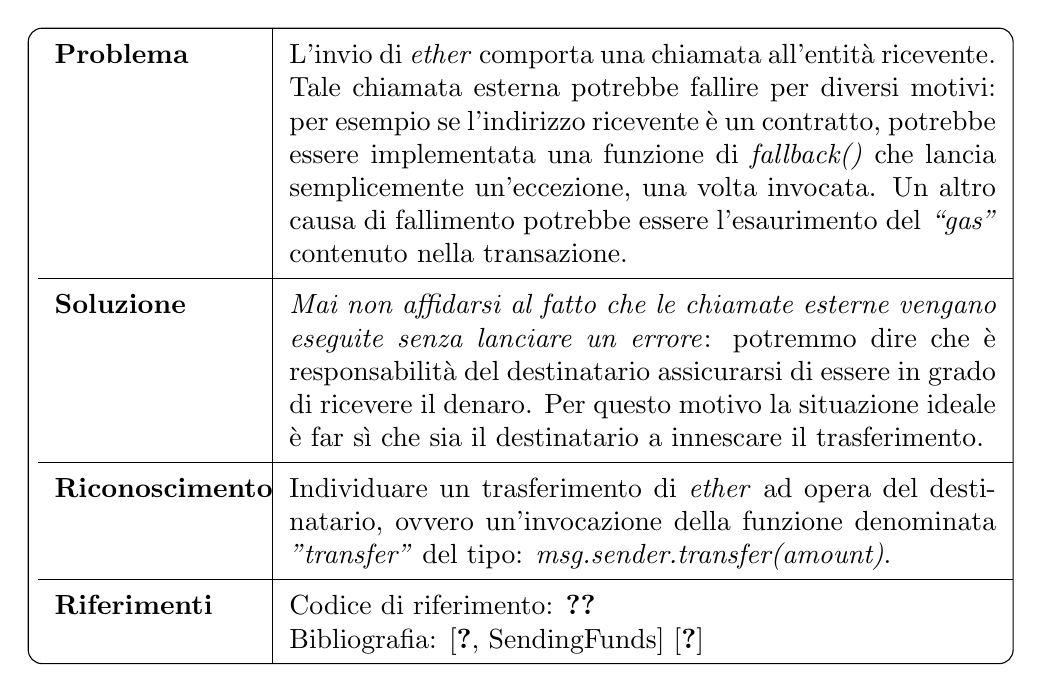
\begin{tikzpicture}
			\node (table) [inner sep=0pt] {
				\def\arraystretch{1.5}
				\begin{tabular}{p{0.21\linewidth} | p{0.74\linewidth}}
					\textbf{Problema} & {L'invio di \textit{ether} comporta una chiamata all'entità ricevente. Tale chiamata esterna potrebbe fallire per diversi motivi: per esempio se l'indirizzo ricevente è un contratto, potrebbe essere implementata una funzione di \textit{fallback()} che lancia semplicemente un'eccezione, una volta invocata. Un altro causa di fallimento potrebbe essere l'esaurimento del \textit{“gas”} contenuto nella transazione.} \\ \hline
					\textbf{Soluzione} & {\textit{Mai non affidarsi al fatto che le chiamate esterne vengano eseguite senza lanciare un errore}: potremmo dire che è responsabilità del destinatario assicurarsi di essere in grado di ricevere il denaro. Per questo motivo la situazione ideale è far sì che sia il destinatario a innescare il trasferimento.} \\ \hline
					\textbf{Riconoscimento} & {Individuare un trasferimento di \textit{ether} ad opera del destinatario, ovvero un'invocazione della funzione denominata \textit{"transfer"} del tipo: \textit{msg.sender.transfer(amount)}.} \\ \hline
					\textbf{Riferimenti} & {Codice di riferimento: \ref{appendix:pull_over_push} \newline Bibliografia: \cite[SendingFunds]{maxwoe} \cite{fravoll}} \\
				\end{tabular}
			};
			\draw [rounded corners=.5em] (table.north west) rectangle (table.south east);
		\end{tikzpicture}
		\caption{Specifiche del Full Payment (Pull Over Push) Pattern}
	\end{table}
}
\newpage
{\subsection{Randomness Pattern}
	La casualità nei sistemi informatici, e soprattutto in Ethereum, è notoriamente difficile da ottenere. Per quanto riguarda Ethereum, la rete è una macchina di Turing deterministica, senza alcuna casualità intrinseca. Un'altra problematica è rappresentata dalla natura pubblica della blockchain: lo stato interno di un contratto, così come l'intera storia di una blockchain, è visibile al pubblico. Pertanto, è difficile trovare una fonte sicura di entropia.\par
	Nonostante ciò, la necessità di casualità è assai elevata. Il \textit{Randomness} pattern propone un meccanismo per consentire a uno smart-contract di generare un numero casuale, appartenente a un intervallo predefinito, in un ambiente deterministico come la blockchain.
	\begin{table}[H]
		\centering
		\begin{tikzpicture}
			\node (table) [inner sep=0pt] {
				\def\arraystretch{1.5}
				\begin{tabular}{p{0.21\linewidth} | p{0.74\linewidth}}
					\textbf{Problema} & {Si immagini uno scenario in cui è necessario l'utilizzo di un fattore di casualità, come ad esempio un gioco d'azzardo.} \\ \hline
					\textbf{Soluzione} & {
					\begin{itemize}[leftmargin=5mm, itemsep=0pt]
						\item \textit{Block Hash PRNG}: l'hash del blocco viene usato come sorgente di casualità;
						\item \textit{Oracle PRNG}: un oracolo assume il ruolo di provider di casualità;
						\item \textit{Collaborative PRNG}: una generazione collaborativa di casualità dentro la blockchain;
					\end{itemize}\vspace{-9mm}
					} \\ \hline
					\textbf{Riconoscimento} & {Data la complessità e la libertà implementativa delle varianti basate sull'oracolo e la generazione collaborativa, si riconosce la variane più semplice basata sull'hash del blocco. L'hash del blocco può essere usato in diversi modi:
					\begin{itemize}[leftmargin=5mm, itemsep=0pt]
						\item \textit{uint(blockhash(block.number-1))}: non utilizzabile per scommesse in quanto facilmente determinabile;
						\item \textit{uint(keccak256(abi.encodePacked(blockhash( block.number-1), seed)))}: il seed viene generato dall'utente e fornito come parametro;
						\item \textit{uint(keccak256(abi.encodePacked(block.timestamp, msg.sender, block.difficulty)))}
					\end{itemize}\vspace{-6mm}
					} \\ \hline
					\textbf{Riferimenti} & {Codice di riferimento: \ref{appendix:randomness} \newline Bibliografia: \cite{fravoll}} \\
				\end{tabular}
			};
			\draw [rounded corners=.5em] (table.north west) rectangle (table.south east);
		\end{tikzpicture}
		\caption{Specifiche del Randomness Pattern}
	\end{table}
}
{\subsection{State Machine Pattern}
	Lo \textit{State Machine} pattern propone un meccanismo per consentire a uno smart-contract di passare, durante la sua esecuzione, attraverso diverse fasi con diverse funzionalità corrispondenti esposte.
	\begin{table}[H]
		\centering
		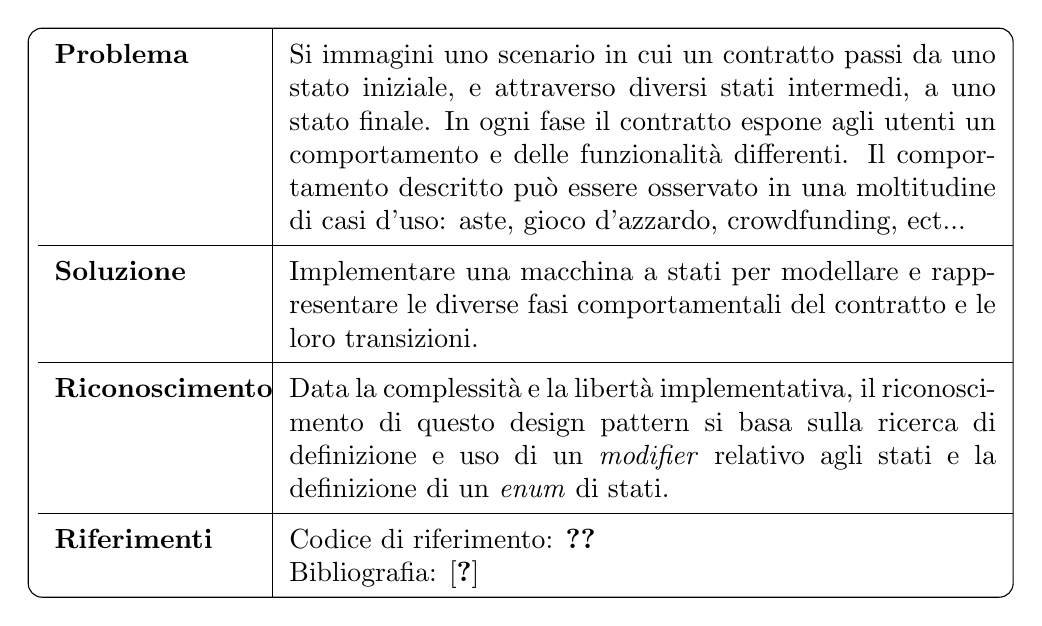
\begin{tikzpicture}
			\node (table) [inner sep=0pt] {
				\def\arraystretch{1.5}
				\begin{tabular}{p{0.21\linewidth} | p{0.74\linewidth}}
					\textbf{Problema} & {Si immagini uno scenario in cui un contratto passi da uno stato iniziale, e attraverso diversi stati intermedi, a uno stato finale. In ogni fase il contratto espone agli utenti un comportamento e delle funzionalità differenti. Il comportamento descritto può essere osservato in una moltitudine di casi d'uso: aste, gioco d'azzardo, crowdfunding, ect...} \\ \hline
					\textbf{Soluzione} & {Implementare una macchina a stati per modellare e rappresentare le diverse fasi comportamentali del contratto e le loro transizioni.} \\ \hline
					\textbf{Riconoscimento} & {Data la complessità e la libertà implementativa, il riconoscimento di questo design pattern si basa sulla ricerca di definizione e uso di un \textit{modifier} relativo agli stati e la definizione di un \textit{enum} di stati.} \\ \hline
					\textbf{Riferimenti} & {Codice di riferimento: \ref{appendix:state_machine} \newline Bibliografia: \cite{maxwoe}} \\
				\end{tabular}
			};
			\draw [rounded corners=.5em] (table.north west) rectangle (table.south east);
		\end{tikzpicture}
		\caption{Specifiche dello State Machine Pattern}
	\end{table}
}
}

{\section{Gas Economic Design Pattern}
	I \textit{Gas Economic design pattern} propongono meccanismi considerabili come \textit{"best practice"} per ridurre il consumo di gas durante l'esecuzione delle funzionalità dello smart-contract. \par
	Per i contratti, Le operazioni con un consumo di gas altamente variabile e imprevedibile costituiscono un problema, in quanto comportano il rischio che le transazioni rimangano senza gas e si ottengano di conseguenza dei comportamenti indesiderati. Pertanto, è auspicabile un fabbisogno di gas basso, stabile e prevedibile.\par
	Si individuano i seguenti design pattern: \textit{Memory Array Building}, \textit{String Equality Comparison} e \textit{Tight Variable Packing}.
	\newpage
	{\subsection{Memory Array Building Pattern}
		Il \textit{Memory Array Building} pattern propone un meccanismo per aggregare e recuperare i dati dallo storage di un contratto in modo efficiente dal punto di vista del consumo di gas.\par	L'interazione con lo storage di un contratto sulla blockchain è una delle operazioni più costose dell'EVM. Pertanto, è necessario memorizzare solo i dati necessari ed evitare, se possibile, la ridondanza. Nei sistemi tradizionali l'unico costo rilevante delle query in uno storage è il tempo, mentre in Ethereum anche semplici interrogazioni possono costare una quantità sostanziale di gas, che ha un riscontro monetario diretto.\par
		Si potrebbe mitigare il costo del gas relativo alla lettura di un dato definendo la variabile contenitore come pubblica, generando così un \textit{getter} in background che permette di accedere gratuitamente al valore della variabile, ma ciò non è sempre applicabile.
		\begin{table}[H]
			\centering
			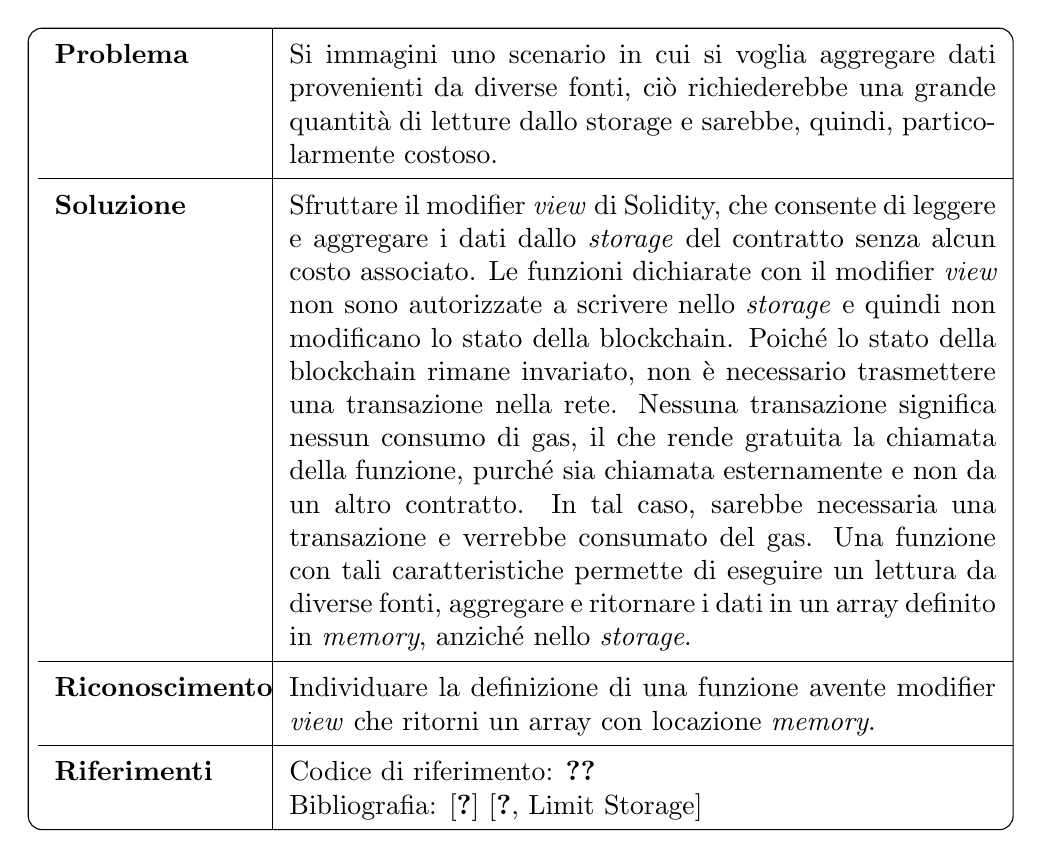
\begin{tikzpicture}
				\node (table) [inner sep=0pt] {
					\def\arraystretch{1.5}
					\begin{tabular}{p{0.21\linewidth} | p{0.74\linewidth}}
						\textbf{Problema} & {Si immagini uno scenario in cui si voglia aggregare dati provenienti da diverse fonti, ciò richiederebbe una grande quantità di letture dallo storage e sarebbe, quindi, particolarmente costoso.} \\ \hline
						\textbf{Soluzione} & {Sfruttare il modifier \textit{view} di Solidity, che consente di leggere e aggregare i dati dallo \textit{storage} del contratto senza alcun costo associato. Le funzioni dichiarate con il modifier \textit{view} non sono autorizzate a scrivere nello \textit{storage} e quindi non modificano lo stato della blockchain. Poiché lo stato della blockchain rimane invariato, non è necessario trasmettere una transazione nella rete. Nessuna transazione significa nessun consumo di gas, il che rende gratuita la chiamata della funzione, purché sia chiamata esternamente e non da un altro contratto. In tal caso, sarebbe necessaria una transazione e verrebbe consumato del gas. Una funzione con tali caratteristiche permette di eseguire un lettura da diverse fonti, aggregare e ritornare i dati in un array definito in \textit{memory}, anziché nello \textit{storage}.} \\ \hline
						\textbf{Riconoscimento} & {Individuare la definizione di una funzione avente modifier \textit{view} che ritorni un array con locazione \textit{memory}.} \\ \hline
						\textbf{Riferimenti} & {Codice di riferimento: \ref{appendix:memory_array_building} \newline Bibliografia: \cite{fravoll} \cite[Limit Storage]{9050163}} \\
					\end{tabular}
				};
				\draw [rounded corners=.5em] (table.north west) rectangle (table.south east);
			\end{tikzpicture}
			\caption{Specifiche del Memory Array Building Pattern}
		\end{table}
	}
	{\subsection{String Equality Comparison Pattern}
		Confrontare delle stringhe nei vari linguaggi di programmazione è spesso un compito banale, vi sono metodi o pacchetti integrati che possono verificare l'uguaglianza di due input con una sola chiamata, ad esempio \textit{String1.equals(String2)} in Java.\par Al momento della stesura del presente documento, Solidity, nella sua versione 0.8.0.0, implementa alcuna soluzione nativa per quest'operazione.\par
		Lo \textit{String Equality Comparison} pattern propone un meccanismo per verificare l'uguaglianza di due stringhe minimizzando il consumo medio del gas per un gran numero di input diversi.
		\begin{table}[H]
			\centering
			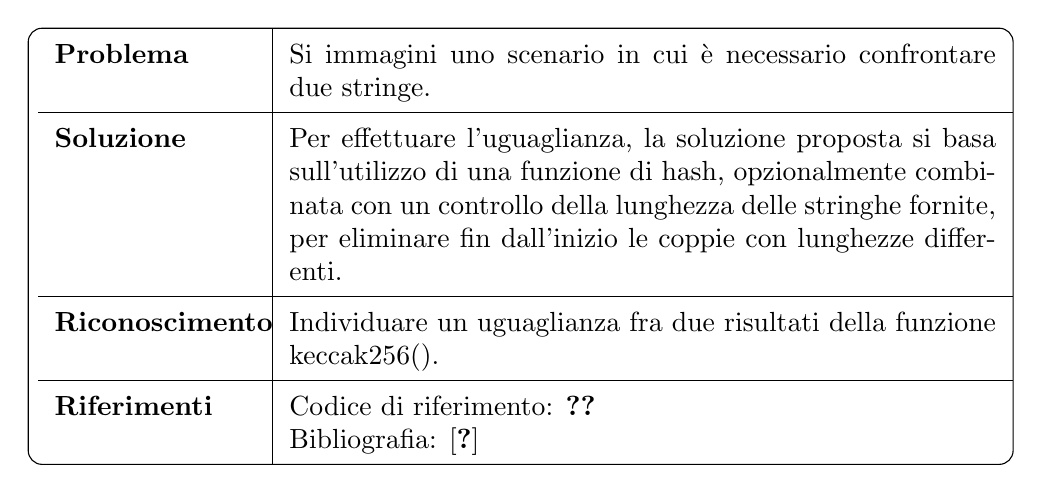
\begin{tikzpicture}
				\node (table) [inner sep=0pt] {
					\def\arraystretch{1.5}
					\begin{tabular}{p{0.21\linewidth} | p{0.74\linewidth}}
						\textbf{Problema} & {Si immagini uno scenario in cui è necessario confrontare due stringe.} \\ \hline
						\textbf{Soluzione} & {Per effettuare l'uguaglianza, la soluzione proposta si basa sull'utilizzo di una funzione di hash, opzionalmente combinata con un controllo della lunghezza delle stringhe fornite, per eliminare fin dall'inizio le coppie con lunghezze differenti.} \\ \hline
						\textbf{Riconoscimento} & {Individuare un uguaglianza fra due risultati della funzione \textit\mbox{keccak256()}.} \\ \hline
						\textbf{Riferimenti} & {Codice di riferimento: \ref{appendix:string_equality_comparison} \newline Bibliografia: \cite{fravoll}} \\
					\end{tabular}
				};
				\draw [rounded corners=.5em] (table.north west) rectangle (table.south east);
			\end{tikzpicture}
			\caption{Specifiche del String Equality Comparison Pattern}
		\end{table}
	}
	{\subsection{Tight Variable Packing Pattern}
	Il \textit{Tight Variable Packing} pattern propone un meccanismo per ottimizzare il consumo di gas nella memorizzazione e nella lettura di variabili di dimensione statica.\par
	Lo storage in Ethereum è una struttura \textit{chiave-valore} con chiavi e valori di 32 byte ciascuno. Quando viene allocato lo storage di un contratto, tutte le variabili di dimensione statica, eccetto le mappature e gli array di dimensione dinamica, vengono memorizzate nello storage una dopo l'altra, nell'ordine in cui sono state dichiarate.\par I tipi di dati più comunemente utilizzati come \textit{byte32}, \textit{uint} e \textit{int} occupano esattamente uno slot da 32 byte, perciò vengono letti o memorizzati con un'unica operazione.\par
	Sarebbe, quindi, ottimale ordinare la dichiarazione dei tipi di dimensione statica più piccola, come \textit{byte16}, \textit{uint8} e così via, in modo che l'EVM possa raggrupparli in un singolo slot da 32 byte e operare su di essi con un'unica operazione, utilizzando meno memoria e risparmiando gas.
	\begin{table}[H]
		\centering
		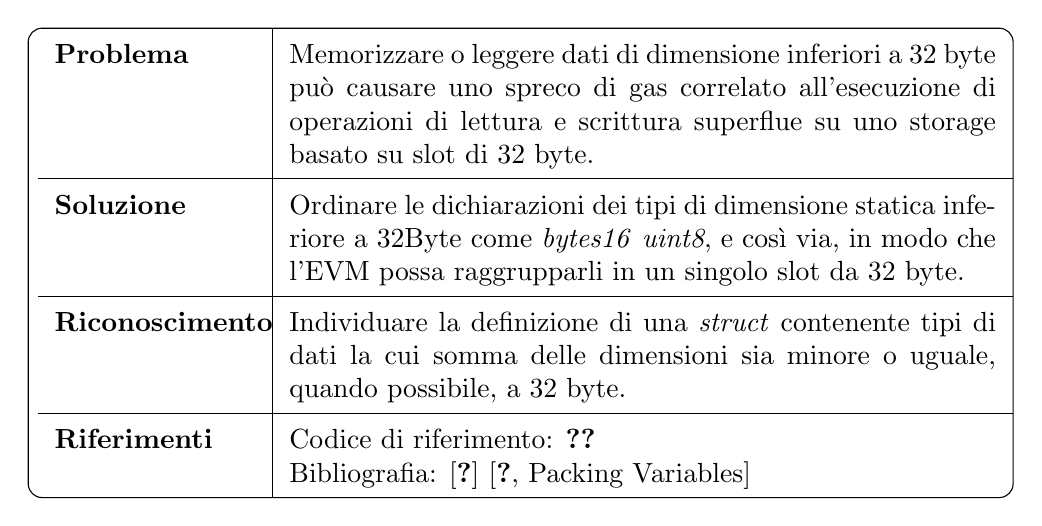
\begin{tikzpicture}
			\node (table) [inner sep=0pt] {
				\def\arraystretch{1.5}
				\begin{tabular}{p{0.21\linewidth} | p{0.74\linewidth}}
					\textbf{Problema} & {Memorizzare o leggere dati di dimensione inferiori a 32 byte può causare uno spreco di gas correlato all'esecuzione di operazioni di lettura e scrittura superflue su uno storage basato su slot di 32 byte.} \\ \hline
					\textbf{Soluzione} & {Ordinare le dichiarazioni dei tipi di dimensione statica inferiore a 32Byte come \textit{bytes16} \textit{uint8}, e così via, in modo che l'EVM possa raggrupparli in un singolo slot da 32 byte.} \\ \hline
					\textbf{Riconoscimento} & {Individuare la definizione di una \textit{struct} contenente tipi di dati la cui somma delle dimensioni sia minore o uguale, quando possibile, a 32 byte.} \\ \hline
					\textbf{Riferimenti} & {Codice di riferimento: \ref{appendix:tight_variable_packing} \newline Bibliografia: \cite{fravoll} \cite[Packing Variables]{9050163}} \\
				\end{tabular}
			};
			\draw [rounded corners=.5em] (table.north west) rectangle (table.south east);
		\end{tikzpicture}
		\caption{Specifiche del Tight Variable Packing Pattern}
	\end{table}
}
}

{\section{Lifecycle Design Pattern}
	I \textit{Lifecycle design pattern} propongono meccanismi per la creazione e la distruzione degli smart-contract. \par
	Si individuano i seguenti design pattern: \textit{Auto Deprecation} e \textit{Mortal}.
	
	{\subsection{Auto Deprecation Pattern}
		L'\textit{Auto Deprecation} pattern propone un meccanismo che, definito uno specifico quanto di tempo, permette di interrompere automaticamente, allo scadere del quanto di tempo, l'esecuzione di specifiche funzionalità del contratto.
		\begin{table}[H]
			\centering
			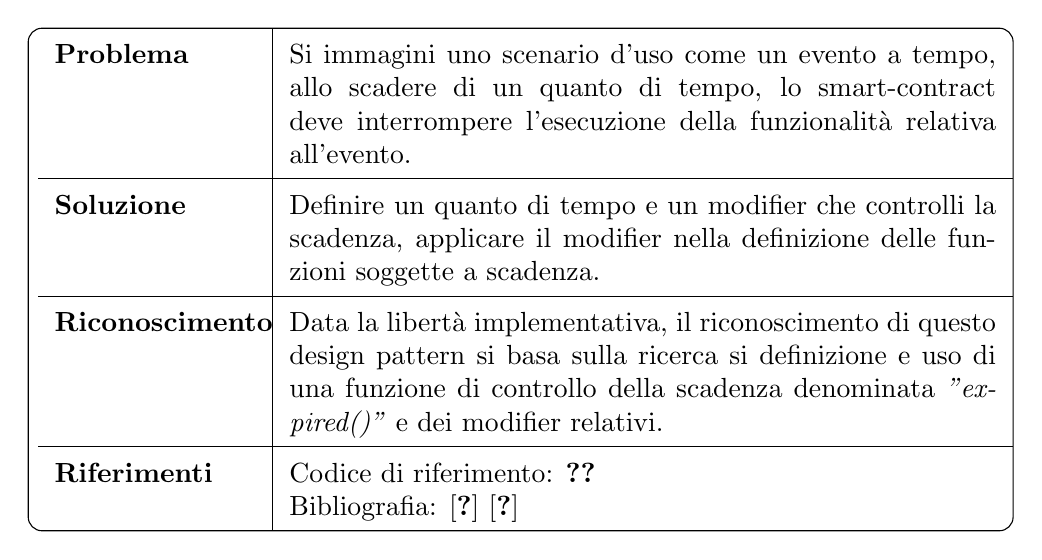
\begin{tikzpicture}
				\node (table) [inner sep=0pt] {
					\def\arraystretch{1.5}
					\begin{tabular}{p{0.21\linewidth} | p{0.74\linewidth}}
						\textbf{Problema} & {Si immagini uno scenario d'uso come un evento a tempo, allo scadere di un quanto di tempo, lo smart-contract deve interrompere l'esecuzione della funzionalità relativa all'evento.} \\ \hline
						\textbf{Soluzione} & {Definire un quanto di tempo e un modifier che controlli la scadenza, applicare il modifier nella definizione delle funzioni soggette a scadenza.} \\ \hline
						\textbf{Riconoscimento} & {Data la libertà implementativa, il riconoscimento di questo design pattern si basa sulla ricerca si definizione e uso di una funzione di controllo della scadenza denominata \textit{"expired()"} e dei modifier relativi.} \\ \hline
						\textbf{Riferimenti} & {Codice di riferimento: \ref{appendix:auto_deprecation} \newline Bibliografia: \cite{maxwoe} \cite{cjgdev}} \\
					\end{tabular}
				};
				\draw [rounded corners=.5em] (table.north west) rectangle (table.south east);
			\end{tikzpicture}
			\caption{Specifiche dell'Auto Deprecation Pattern}
		\end{table}
	}
	{\subsection{Mortal Pattern}
		Il \textit{Mortal} pattern propone un meccanismo per terminare e distruggere un contratto.\par
		Poiché è la distruzione di un contratto è un operazione critica, la funzionalità è riservata al proprietario del contratto e per questo motivo l'accesso a tale funzione viene spesso gestito attraverso un \textit{Authorization pattern design}.
		\begin{table}[H]
			\centering
			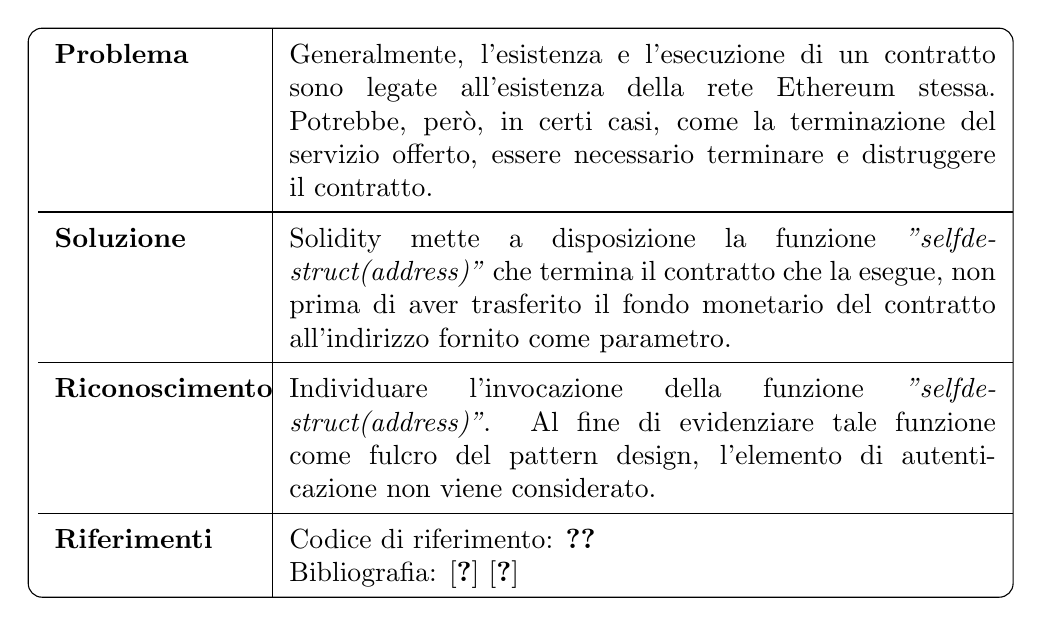
\begin{tikzpicture}
				\node (table) [inner sep=0pt] {
					\def\arraystretch{1.5}
					\begin{tabular}{p{0.21\linewidth} | p{0.74\linewidth}}
						\textbf{Problema} & {Generalmente, l'esistenza e l'esecuzione di un contratto sono legate all'esistenza della rete Ethereum stessa. Potrebbe, però, in certi casi, come la terminazione del servizio offerto, essere necessario terminare e distruggere il contratto.} \\ \hline
						\textbf{Soluzione} & {Solidity mette a disposizione la funzione \textit{"selfdestruct(address)"} che termina il contratto che la esegue, non prima di aver trasferito il fondo monetario del contratto all'indirizzo fornito come parametro.} \\ \hline
						\textbf{Riconoscimento} & {Individuare l'invocazione della funzione \textit{"selfdestruct(address)"}. Al fine di evidenziare tale funzione come fulcro del pattern design, l'elemento di autenticazione non viene considerato.} \\ \hline
						\textbf{Riferimenti} & {Codice di riferimento: \ref{appendix:mortal} \newline Bibliografia: \cite{maxwoe}} \cite{cjgdev} \\
					\end{tabular}
				};
				\draw [rounded corners=.5em] (table.north west) rectangle (table.south east);
			\end{tikzpicture}
			\caption{Specifiche del Mortal Pattern}
		\end{table}
	}
}

{\section{Maintenance Design Pattern}
	I \textit{Maintenance design pattern} propongono, definendo modalità con cui strutturare il codice, meccanismi e funzionalità utili per uno smart-contract. \par
	Si individuano i seguenti design pattern: \textit{Data Segregation}, \textit{Register} e \textit{Relay}.
	
	{\subsection{Data Segregation Pattern}
		Il \textit{Data Segregation} pattern, noto anche come \textit{Eternal Storage}, propone un meccanismo atto a segmentare la logica di un contratto e i suoi dati, al fine di evitare, in seguito all'aggiornamento del contratto, costose migrazioni di dati.
		\begin{table}[H]
			\centering
			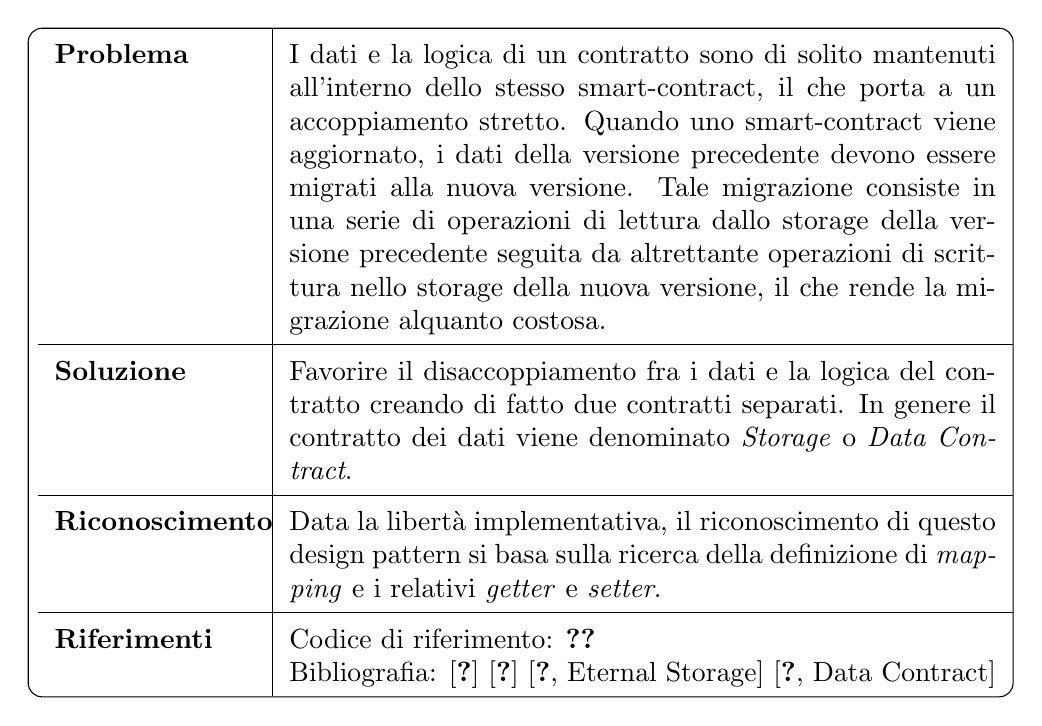
\begin{tikzpicture}
				\node (table) [inner sep=0pt] {
					\def\arraystretch{1.5}
					\begin{tabular}{p{0.21\linewidth} | p{0.74\linewidth}}
						\textbf{Problema} & {I dati e la logica di un contratto sono di solito mantenuti all'interno dello stesso smart-contract, il che porta a un accoppiamento stretto. Quando uno smart-contract viene aggiornato, i dati della versione precedente devono essere migrati alla nuova versione. Tale migrazione consiste in una serie di operazioni di lettura dallo storage della versione precedente seguita da altrettante operazioni di scrittura nello storage della nuova versione, il che rende la migrazione alquanto costosa.} \\ \hline
						\textbf{Soluzione} & {Favorire il disaccoppiamento fra i dati e la logica del contratto creando di fatto due contratti separati. In genere il contratto dei dati viene denominato \textit{Storage} o \textit{Data Contract}.} \\ \hline
						\textbf{Riconoscimento} & {Data la libertà implementativa, il riconoscimento di questo design pattern si basa sulla ricerca della definizione di \textit{mapping} e i relativi \textit{getter} e \textit{setter}.} \\ \hline
						\textbf{Riferimenti} & {Codice di riferimento: \ref{appendix:data_segregation} \newline Bibliografia: \cite{maxwoe} \cite{cjgdev} \cite[Eternal Storage]{fravoll} \cite[Data Contract]{9050163}} \\
					\end{tabular}
				};
				\draw [rounded corners=.5em] (table.north west) rectangle (table.south east);
			\end{tikzpicture}
			\caption{Specifiche del Data Segregation Pattern}
		\end{table}
	}
\newpage
	{\subsection{Register e Relay Pattern}
		Sia il \textit{Register} pattern  sia il \textit{Relay} pattern, noto anche come \textit{Proxy Delegate}, propongono un meccanismo per disaccoppiare la logica del contratto dal canale di comunicazione con l'utente, ovvero l'indirizzo con cui quest'ultimo interagisce con il contratto stesso.\par
		I due design pattern seppur strutturalmente diversi si basano entrambi sulla delegazione delle chiamate ricevute. Assumono il ruolo di mediatore fra l'utente e l'attuale logica del contratto.
		
		\begin{table}[H]
			\centering
			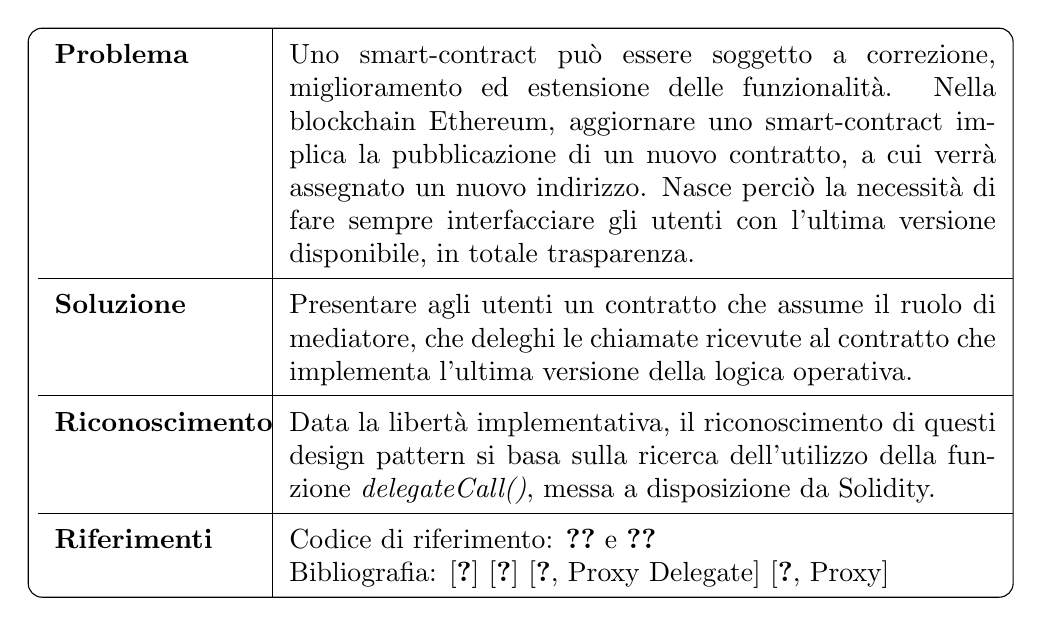
\begin{tikzpicture}
				\node (table) [inner sep=0pt] {
					\def\arraystretch{1.5}
					\begin{tabular}{p{0.21\linewidth} | p{0.74\linewidth}}
						\textbf{Problema} & {Uno smart-contract può essere soggetto a correzione, miglioramento ed estensione delle funzionalità. Nella blockchain Ethereum, aggiornare uno smart-contract implica la pubblicazione di un nuovo contratto, a cui verrà assegnato un nuovo indirizzo. Nasce perciò la necessità di fare sempre interfacciare gli utenti con l'ultima versione disponibile, in totale trasparenza.} \\ \hline
						\textbf{Soluzione} & {Presentare agli utenti un contratto che assume il ruolo di mediatore, che deleghi le chiamate ricevute al contratto che implementa l'ultima versione della logica operativa.} \\ \hline
						\textbf{Riconoscimento} & {Data la libertà implementativa, il riconoscimento di questi design pattern si basa sulla ricerca dell'utilizzo della funzione \textit{delegateCall()}, messa a disposizione da Solidity.} \\ \hline
						\textbf{Riferimenti} & {Codice di riferimento: \ref{appendix:register} e \ref{appendix:relay} \newline Bibliografia: \cite{maxwoe} \cite{cjgdev} \cite[Proxy Delegate]{fravoll} \cite[Proxy]{9050163}} \\
					\end{tabular}
				};
				\draw [rounded corners=.5em] (table.north west) rectangle (table.south east);
			\end{tikzpicture}
			\caption{Specifiche del Register/Relay Pattern}
		\end{table}
	}
}
\newpage
{\section{Security Design Pattern}
	I \textit{Security design pattern} propongono meccanismi utili a mitigare le vulnerabilità di sicurezza note. \par
	Si individuano i seguenti design pattern: \textit{Balance Limit}, \textit{Check Effects Interactions}, \textit{Emergency Stop}, \textit{Mutex}, \textit{Rate Limit} e \textit{Rejector}.
	
	{\subsection{Balance Limit Pattern}
		Il \textit{Balance Limit} pattern propone un meccanismo per contenere i possibili danni o compromissioni gli possono incorrere in caso di bug nel codice o exploit di vulnerabilità non ancora identificate e mitigate.\par
		Il meccanismo proposto dal pattern è molto basilare: imporre un tetto massimo al bilancio delle utenze.
		\begin{table}[H]
			\centering
			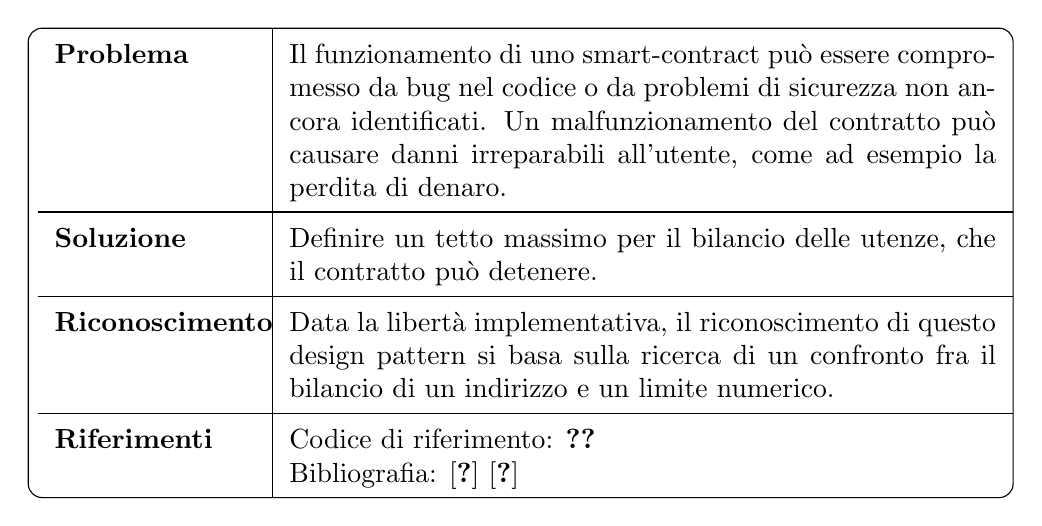
\begin{tikzpicture}
				\node (table) [inner sep=0pt] {
					\def\arraystretch{1.5}
					\begin{tabular}{p{0.21\linewidth} | p{0.74\linewidth}}
						\textbf{Problema} & {Il funzionamento di uno smart-contract può essere compromesso da bug nel codice o da problemi di sicurezza non ancora identificati. Un malfunzionamento del contratto può causare danni irreparabili all'utente, come ad esempio la perdita di denaro.} \\ \hline
						\textbf{Soluzione} & {Definire un tetto massimo per il bilancio delle utenze, che il contratto può detenere.} \\ \hline
						\textbf{Riconoscimento} & {Data la libertà implementativa, il riconoscimento di questo design pattern si basa sulla ricerca di un confronto fra il bilancio di un indirizzo e un limite numerico.} \\ \hline
						\textbf{Riferimenti} & {Codice di riferimento: \ref{appendix:balance_limit} \newline Bibliografia: \cite{maxwoe} \cite{8327565}} \\
					\end{tabular}
				};
				\draw [rounded corners=.5em] (table.north west) rectangle (table.south east);
			\end{tikzpicture}
			\caption{Specifiche del Balance Limit Pattern}
		\end{table}
	}
\newpage
	{\subsection{Check Effects Interactions Pattern}
		Il \textit{Check Effects Interactions} pattern propone un meccanismo per mitigare possibili manipolazioni di stato e dirottamenti del controllo di flusso che possono 
		avvenire quando il contratto comunica con un'entità esterno, come ad esempio un utente o un altro smart-contract.
		\begin{table}[H]
			\centering
			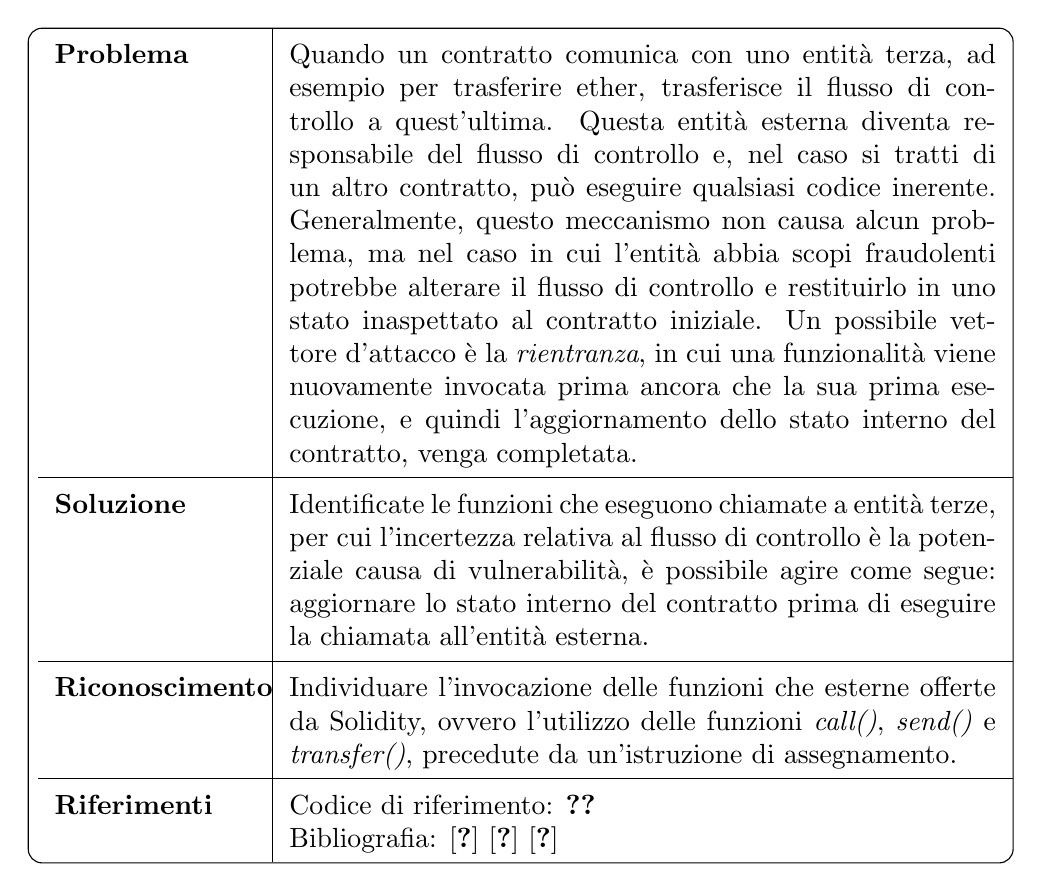
\begin{tikzpicture}
				\node (table) [inner sep=0pt] {
					\def\arraystretch{1.5}
					\begin{tabular}{p{0.21\linewidth} | p{0.74\linewidth}}
						\textbf{Problema} & {Quando un contratto comunica con uno entità terza, ad esempio per trasferire ether, trasferisce il flusso di controllo a quest'ultima. Questa entità esterna diventa responsabile del flusso di controllo e, nel caso si tratti di un altro contratto, può eseguire qualsiasi codice inerente. Generalmente, questo meccanismo non causa alcun problema, ma nel caso in cui l'entità abbia scopi fraudolenti potrebbe alterare il flusso di controllo e restituirlo in uno stato inaspettato al contratto iniziale. Un possibile vettore d'attacco è la \textit{rientranza}, in cui una funzionalità viene nuovamente invocata prima ancora che la sua prima esecuzione, e quindi l'aggiornamento dello stato interno del contratto, venga completata.} \\ \hline
						\textbf{Soluzione} & {Identificate le funzioni che eseguono chiamate a entità terze, per cui l'incertezza relativa al flusso di controllo è la potenziale causa di vulnerabilità, è possibile agire come segue: aggiornare lo stato interno del contratto prima di eseguire la chiamata all'entità esterna.} \\ \hline
						\textbf{Riconoscimento} & {Individuare l'invocazione delle funzioni che esterne offerte da Solidity, ovvero l'utilizzo delle funzioni \textit{call()}, \textit{send()} e \textit{transfer()}, precedute da un'istruzione di assegnamento.} \\ \hline
						\textbf{Riferimenti} & {Codice di riferimento: \ref{appendix:check_effects_interactions} \newline Bibliografia: \cite{maxwoe} \cite{fravoll} \cite{8327565}} \\
					\end{tabular}
				};
				\draw [rounded corners=.5em] (table.north west) rectangle (table.south east);
			\end{tikzpicture}
			\caption{Specifiche Check Effects Interactions Pattern}
		\end{table}
	}

	{\subsection{Emergency Stop Pattern}
	Nella blockchain Ethereum, una volta pubblicato un contratto, quest'ultimo viene eseguito autonomamente senza alcun controllo sulla sua esecuzione. Ciò implica che non è possibile interrompere l'esecuzione totale o parziale delle funzionalità del contratto in caso di bug o problemi di sicurezza.\par L'\textit{Emergency Stop} pattern, noto anche come \textit{Circuit Breaker}, propone un meccanismo per implementare un interruttore software, capace di abilitare o disabilitare l'esecuzione parziale o totale delle funzionalità del contratto.\par Poiché l'azionamento dell'interruttore è un operazione critica, la funzionalità è riservata al proprietario del contratto e per questo motivo l'accesso a tale metodo viene spesso gestito attraverso un \textit{Authorization pattern design}.
	\begin{table}[H]
		\centering
		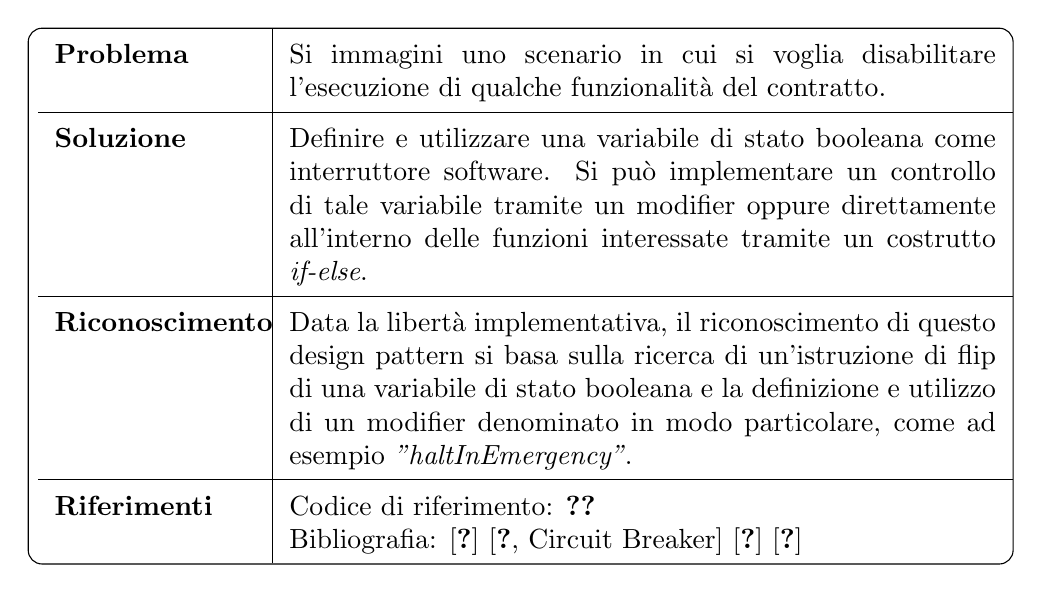
\begin{tikzpicture}
			\node (table) [inner sep=0pt] {
				\def\arraystretch{1.5}
				\begin{tabular}{p{0.21\linewidth} | p{0.74\linewidth}}
					\textbf{Problema} & {Si immagini uno scenario in cui si voglia disabilitare l'esecuzione di qualche funzionalità del contratto.} \\ \hline
					\textbf{Soluzione} & {Definire e utilizzare una variabile di stato booleana come interruttore software. Si può implementare un controllo di tale variabile tramite un modifier oppure direttamente all'interno delle funzioni interessate tramite un costrutto \textit{if-else}.} \\ \hline
					\textbf{Riconoscimento} & {Data la libertà implementativa, il riconoscimento di questo design pattern si basa sulla ricerca di un'istruzione di flip di una variabile di stato booleana e la definizione e utilizzo di un modifier denominato in modo particolare, come ad esempio \textit{"haltInEmergency"}.} \\ \hline
					\textbf{Riferimenti} & {Codice di riferimento: \ref{appendix:emergency_stop} \newline Bibliografia: \cite{maxwoe} \cite[Circuit Breaker]{cjgdev} \cite{fravoll} \cite{8327565}} \\
				\end{tabular}
			};
			\draw [rounded corners=.5em] (table.north west) rectangle (table.south east);
		\end{tikzpicture}
		\caption{Specifiche dell'Emergency Stop Pattern}
	\end{table}
}
	{\subsection{Mutex Pattern}
	 Un attacco basato sulla rientranza consiste nell'invocare nuovamente una funzionalità prima ancora che la sua prima esecuzione, e quindi l'aggiornamento dello stato interno del contratto, venga completata.\par
	Il \textit{Mutex} pattern propone un meccanismo per mitigare le possibili vulnerabilità di \textit{rientranza} basato sul concetto di \textit{semaforo con mutua esclusione}.
	\begin{table}[H]
		\centering
		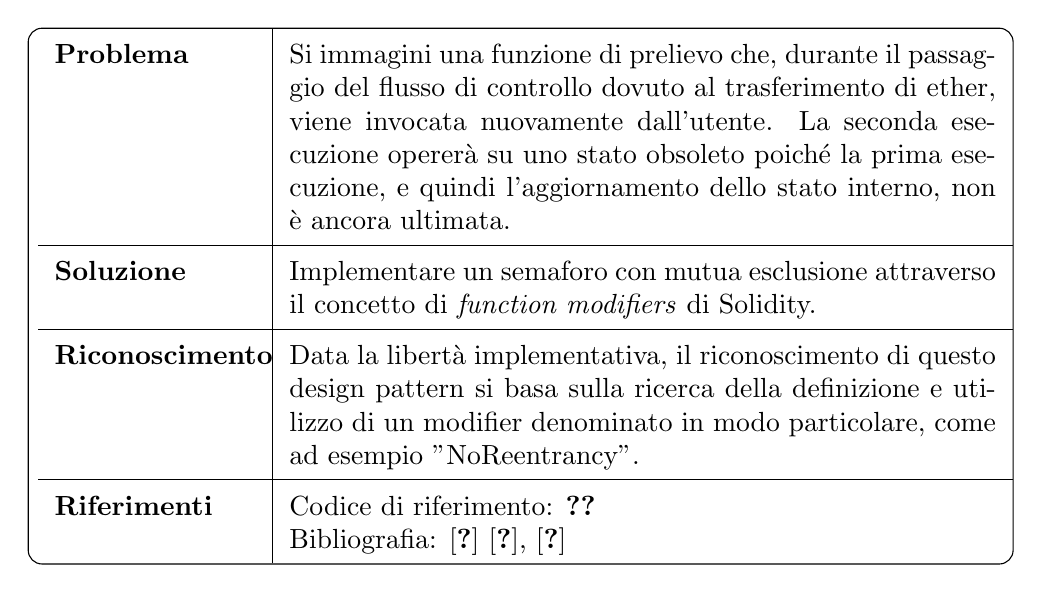
\begin{tikzpicture}
			\node (table) [inner sep=0pt] {
				\def\arraystretch{1.5}
				\begin{tabular}{p{0.21\linewidth} | p{0.74\linewidth}}
					\textbf{Problema} & {Si immagini una funzione di prelievo che, durante il passaggio del flusso di controllo dovuto al trasferimento di ether, viene invocata nuovamente dall'utente. La seconda esecuzione opererà su uno stato obsoleto poiché la prima esecuzione, e quindi l'aggiornamento dello stato interno, non è ancora ultimata.} \\ \hline
					\textbf{Soluzione} & {Implementare un semaforo con mutua esclusione attraverso il concetto di \textit{function modifiers} di Solidity.} \\ \hline
					\textbf{Riconoscimento} & {Data la libertà implementativa, il riconoscimento di questo design pattern si basa sulla ricerca della definizione e utilizzo di un modifier denominato in modo particolare, come ad esempio \textit\mbox{"NoReentrancy"}.} \\ \hline
					\textbf{Riferimenti} & {Codice di riferimento: \ref{appendix:mutex} \newline Bibliografia: \cite{maxwoe} \cite{cjgdev}, \cite{8327565}} \\
				\end{tabular}
			};
			\draw [rounded corners=.5em] (table.north west) rectangle (table.south east);
		\end{tikzpicture}
		\caption{Specifiche del Mutex Pattern}
	\end{table}
}
	{\subsection{Rate Limit Pattern}
	Il \textit{Rate Limit} pattern propone un meccanismo per mitigare un possibile calo di prestazioni del contratto dovuto a un attaccato basato su una rapida successione di richieste di una particolare funzionalità.
	\begin{table}[H]
		\centering
		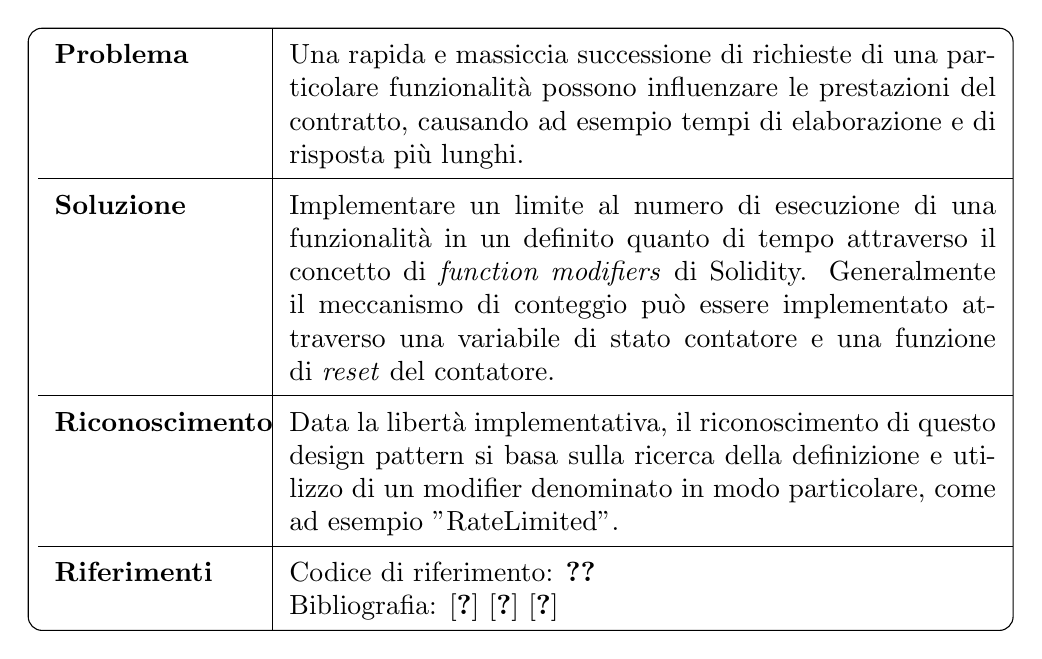
\begin{tikzpicture}
			\node (table) [inner sep=0pt] {
				\def\arraystretch{1.5}
				\begin{tabular}{p{0.21\linewidth} | p{0.74\linewidth}}
					\textbf{Problema} & {Una rapida e massiccia successione di richieste di una particolare funzionalità possono influenzare le prestazioni del contratto, causando ad esempio tempi di elaborazione e di risposta più lunghi.} \\ \hline
					\textbf{Soluzione} & {Implementare un limite al numero di esecuzione di una funzionalità in un definito quanto di tempo attraverso il concetto di \textit{function modifiers} di Solidity. Generalmente il meccanismo di conteggio può essere implementato attraverso una variabile di stato contatore e una funzione di \textit{reset} del contatore. } \\ \hline
					\textbf{Riconoscimento} & {Data la libertà implementativa, il riconoscimento di questo design pattern si basa sulla ricerca della definizione e utilizzo di un modifier denominato in modo particolare, come ad esempio \textit\mbox{"RateLimited"}.} \\ \hline
					\textbf{Riferimenti} & {Codice di riferimento: \ref{appendix:rate_limit} \newline Bibliografia: \cite{maxwoe} \cite{cjgdev} \cite{8327565}} \\
				\end{tabular}
			};
			\draw [rounded corners=.5em] (table.north west) rectangle (table.south east);
		\end{tikzpicture}
		\caption{Specifiche del Rate Limit Pattern}
	\end{table}
}
	{\subsection{Rejector Pattern}
	Il \textit{Rejector} pattern propone un meccanismo per mantenere attivo un contratto ma 
	rifiutare le richieste pervenute.\par
	Questo design pattern può essere usato in combinazione con il disaccoppiamento fra logica e indirizzo, quindi in combinazione con il \textit{Relay} o \textit{Register} pattern.
	\begin{table}[H]
		\centering
		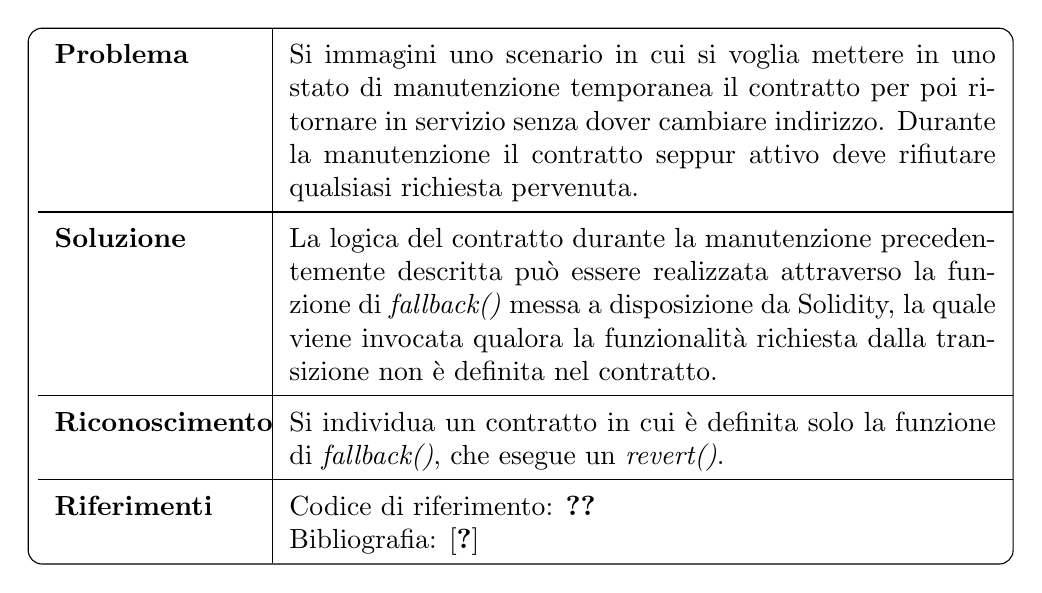
\begin{tikzpicture}
			\node (table) [inner sep=0pt] {
				\def\arraystretch{1.5}
				\begin{tabular}{p{0.21\linewidth} | p{0.74\linewidth}}
					\textbf{Problema} & {Si immagini uno scenario in cui si voglia mettere in uno stato di manutenzione temporanea il contratto per poi ritornare in servizio senza dover cambiare indirizzo. Durante la manutenzione il contratto seppur attivo deve rifiutare qualsiasi richiesta pervenuta.} \\ \hline
					\textbf{Soluzione} & {La logica del contratto durante la manutenzione precedentemente descritta può essere realizzata attraverso la funzione di \textit{fallback()} messa a disposizione da Solidity, la quale viene invocata qualora la funzionalità richiesta dalla transizione non è definita nel contratto.} \\ \hline
					\textbf{Riconoscimento} & {Si individua un contratto in cui è definita solo la funzione di \textit{fallback()}, che esegue un \textit{revert()}.} \\ \hline
					\textbf{Riferimenti} & {Codice di riferimento: \ref{appendix:rejector} \newline Bibliografia: \cite{cjgdev}} \\
				\end{tabular}
			};
			\draw [rounded corners=.5em] (table.north west) rectangle (table.south east);
		\end{tikzpicture}
		\caption{Specifiche del Rejector Pattern}
	\end{table}
}
}